
To enable the agents to communicate with each either in a multi-agent system a blackboard communication system is introduced. 
The blackboard system is essentially a node containing all the information for agents to share with each other. 
The information can be separated using different topics depending on the internal hierarchy of the multi-agent system. 
As doing so the agents can be split into groups and only specific information will be shared while still maintaining information sharing inside the groups.

\begin{figure}[ht]
    \centering
    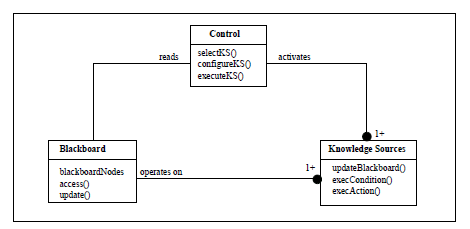
\includegraphics[scale=1.0]{blackboard.png}
    \caption[Blackboard communication]{Blackboard communication}
\end{figure}
